\documentclass{beamer}
%\usepackage[osf,sc]{mathpazo}
\usepackage{eulervm}
\usepackage{tikz}
\usetikzlibrary{arrows,shapes,backgrounds}
\usepackage[backend=biber,style=authoryear-comp,sorting=none]{biblatex}
\addbibresource{../Bibliography.bib}
\usetheme{boxes}
\usecolortheme{rose}
%\usefonttheme{serif}
\setbeamertemplate{navigation symbols}{}

\usepackage{graphicx}
\DeclareMathOperator*{\argmax}{arg\,max}
\DeclareMathOperator*{\argmin}{arg\,min}
\DeclareMathOperator*{\Var}{Var}
\DeclareMathOperator*{\COV}{Cov}

\newcommand{\expSym}{{E}}
\newcommand{\E}[1]{\ensuremath{\expSym\left(#1\right)}}
\newcommand{\prob}[1]{\ensuremath{\Pr\left(#1\right)}}
\newcommand{\T}{T}
\newcommand{\Cov}[2]{\ensuremath{\COV(#1, #2)}}
\newcommand{\bottomcite}[1]{\vspace*{\fill} {\scriptsize \parencite{#1}}}

\renewcommand{\vec}[1]{\ensuremath{#1}}

\usepackage{amsmath}
\usepackage{amssymb}
\usepackage{amsthm}
\usepackage{multirow}
\usepackage{mathtools}

\setbeamertemplate{footline}[frame number]

\title{Analysis of Markovian Population Models}
\subtitle{Dissertation Defense}
\author{Michael Backenk\"{o}hler}
\institute{Saarland Informatics Campus}
\date{September 20, 2022}

\begin{document}

\tikzstyle{every picture}+=[remember picture]
\tikzstyle{na} = [baseline=-.5ex]

\begin{frame}
\titlepage
\end{frame}

\begin{frame}{Motivation}
  \begin{itemize}
    \item Example
    \item list other applications: queueing, metabolic networks, switches etc.
  \end{itemize}
\end{frame}

\begin{frame}{Markovian Population Models}{Semantics}
  \begin{itemize}
    \item counting agents / population size
    \item continuous time
    \item exponential jump times / CTMC dynamics
    \item example: birth-death process
  \end{itemize}
\end{frame}

\section{Markovian Population Models}
\begin{frame}{Markovian Population Models}{Stationary Distribution -- Foster-Lyapunov Functions}
    \begin{itemize}
        \item ergodic chains converge to unique distribution
        \item how does this distribution look like for infinite state-spaces?
        \item use Foster-Lyapunov function to bound sets
        \item locally augment functions for tighter sets / bounds
    \end{itemize}
\end{frame}

\begin{frame}{Markovian Population Models}{Moment Dynamics}
  \begin{itemize}
    \item alternative approach: look at moments instead of states
    \item expected values, e.g. $\E{X}, \E{X^2}$
    \begin{figure}
        \centering
    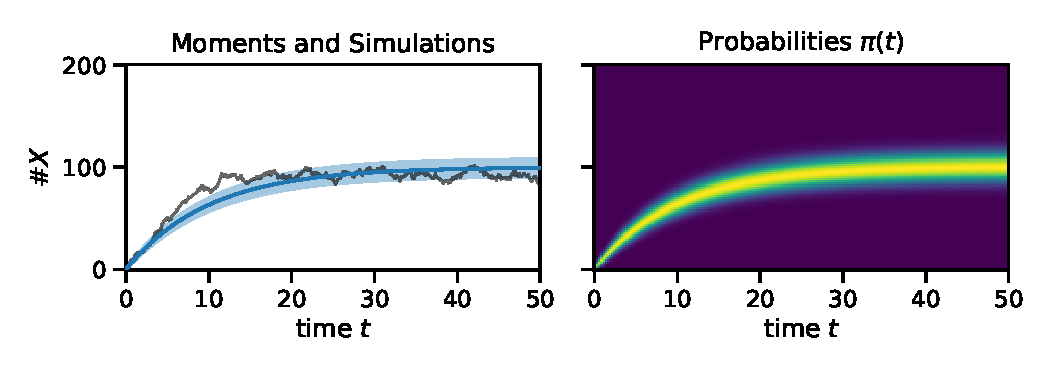
\includegraphics[scale=.4]{../gfx/momsandprobs.pdf}
    \end{figure}
    \item Moment formula
        \begin{equation*}
            \frac{d}{dt}\E{f({\vec{ X}}_t)} = \sum_{j=1}^{n_R}\E{\left(f({\vec X_t +
            \vec{v}_j}) - f(\vec X_t)\right)\alpha_j(\vec X_t)}
        \end{equation*}
    \item ODE system not closed
  \end{itemize}
\end{frame}

\begin{frame}{Markovian Population Models}{Martingale Process}
    \begin{itemize}
    \item multiply time-weighting: $w(t)=t^k$, $k\in\mathbb{N}$ or $w(t)=\exp(\lambda t)$
    \item analytic integration and resulting martingale process
        \begin{equation*}
            \begin{split}
            Z_T\coloneqq&\,w(T)f(\vec X_T) - w(0)f(\vec X_{0}) -
            \int_{0}^T\frac{dw(t)}{dt}f(\vec X_t)\,dt\\
            &-\sum_{j=1}^{n_R}\int_{0}^Tw(t)
                 (f(\vec X_t+\vec v_j) - f(\vec X_t))\alpha_j(\vec X_t)\,dt
         \end{split}
        \end{equation*}
    \item known expectation: $\E{Z_T}=0$, $\forall T\geq 0$
  \end{itemize}
\end{frame}

\section{Bounding Mean First-Passage Times}
\begin{frame}{Bounding Mean First-Passage Times}{Martingale Process and Linear Moment Constraints}
  \begin{itemize}
      \item expected occupation time and exit measures (in relation to expectation of the martingale)
    \begin{figure}
        \centering
        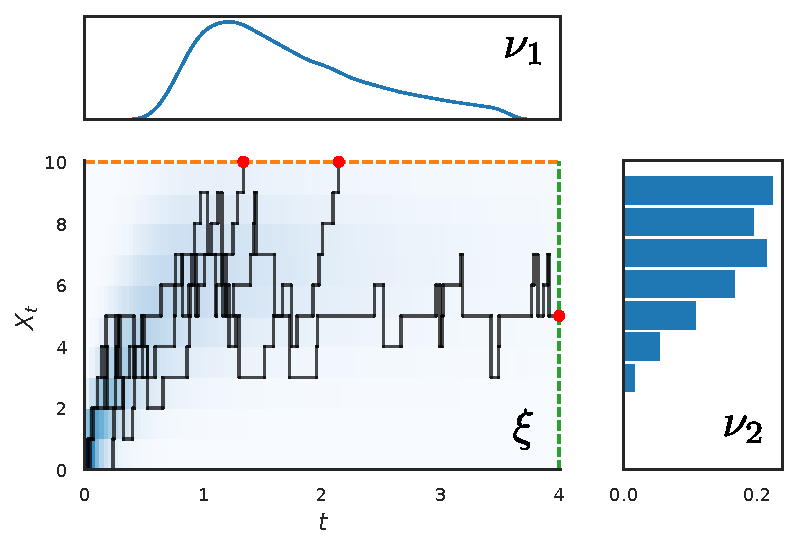
\includegraphics[scale=.4]{../gfx/decomp1.pdf}
    \end{figure}
    \item $0=\E{ Z_T }$ is a linear moment constraint constraint on $\nu_1$, $\nu_2$, and $\xi$ ($w(t)=t^k$) (TODO: integrate moms and figure)
  \end{itemize}

\bottomcite{backenkohler2019bounding}
\end{frame}

\begin{frame}{Bounding Mean First-Passage Times}{Moment Matrices and Semi-Definite Programs}
  \begin{itemize}
    \item semi-definite moment constraints (positive variance as example)
    \item hint at localizing matrices
  \end{itemize}
\bottomcite{backenkohler2019bounding}
\end{frame}

\begin{frame}{Bounding Mean First-Passage Times}{Results and Practical Issues}
  \begin{itemize}
    \item moment problems are inherently stiff
    \item 
    \item some examples
  \end{itemize}
\bottomcite{backenkohler2019bounding}
\end{frame}

\begin{frame}{Bounding Mean First-Passage Times}{Hausdorff Constraints and Linear Programs}
  \begin{itemize}
    \item linear constraints possible if domains (time and space) are finite
    \item 1D visualization of Hausdorff constraints
  \end{itemize}
\end{frame}

\section{Linear Control Variates}
\begin{frame}{Linear Control Variates}{Using Correlated RVs with Known Expected Value}
    \begin{columns}
        \begin{column}{.6\textwidth}
          \begin{itemize}
            \item segue: use the same martingale constraints to enhance MC estimation
            \item $\E{X_T}=\E{X_T}+b\E{Z_T}$
            \item use correlations between target RV and martingales (linear regression, i.e.\ control variates)
          \end{itemize}
        \end{column}
        \begin{column}{.38\textwidth}
            \begin{figure}
                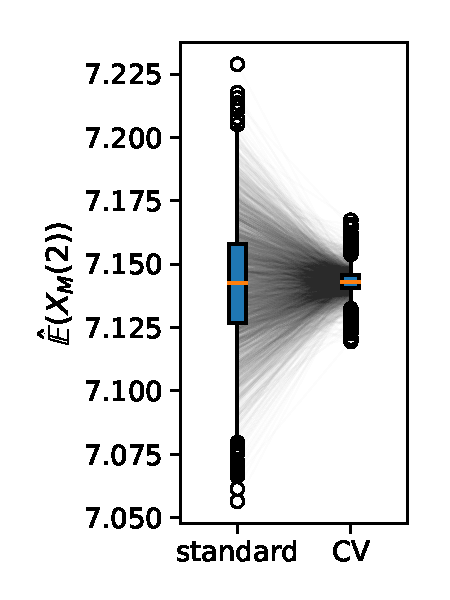
\includegraphics[width=\textwidth]{../gfx/reduction.pdf}
            \end{figure}
        \end{column}
    \end{columns}
    \bottomcite{backenkohler2019control}
\end{frame}

\begin{frame}{Linear Control Variates}{Finding Efficient Sets of Control Variates}
  \begin{itemize}
    \item time-weighting has a large influence on the correlation
    \item Infinitely many possibilities (cost needs to be controlled though)
    \item variates can be highly redundant (correlated) and incur an additional cost
    \item Alg.~1: Tighten an initial proposal set
    \item Alg.~2: Re-sample promising candidates
  \end{itemize}
    \bottomcite{backenkohler2019control,backenkohler2021variance}
\end{frame}

\begin{frame}{Linear Control Variates}{Selection Algorithms}
\end{frame}

\begin{frame}{Linear Control Variates}{Results}
  \begin{itemize}
    \item best example?
  \end{itemize}
\end{frame}

\section{State-Space Aggregation}
\begin{frame}{State-Space Aggregation}{Treating Hyper-Cubes of States as One}
    \begin{columns}
        \begin{column}{.4\textwidth}
            \begin{figure}
            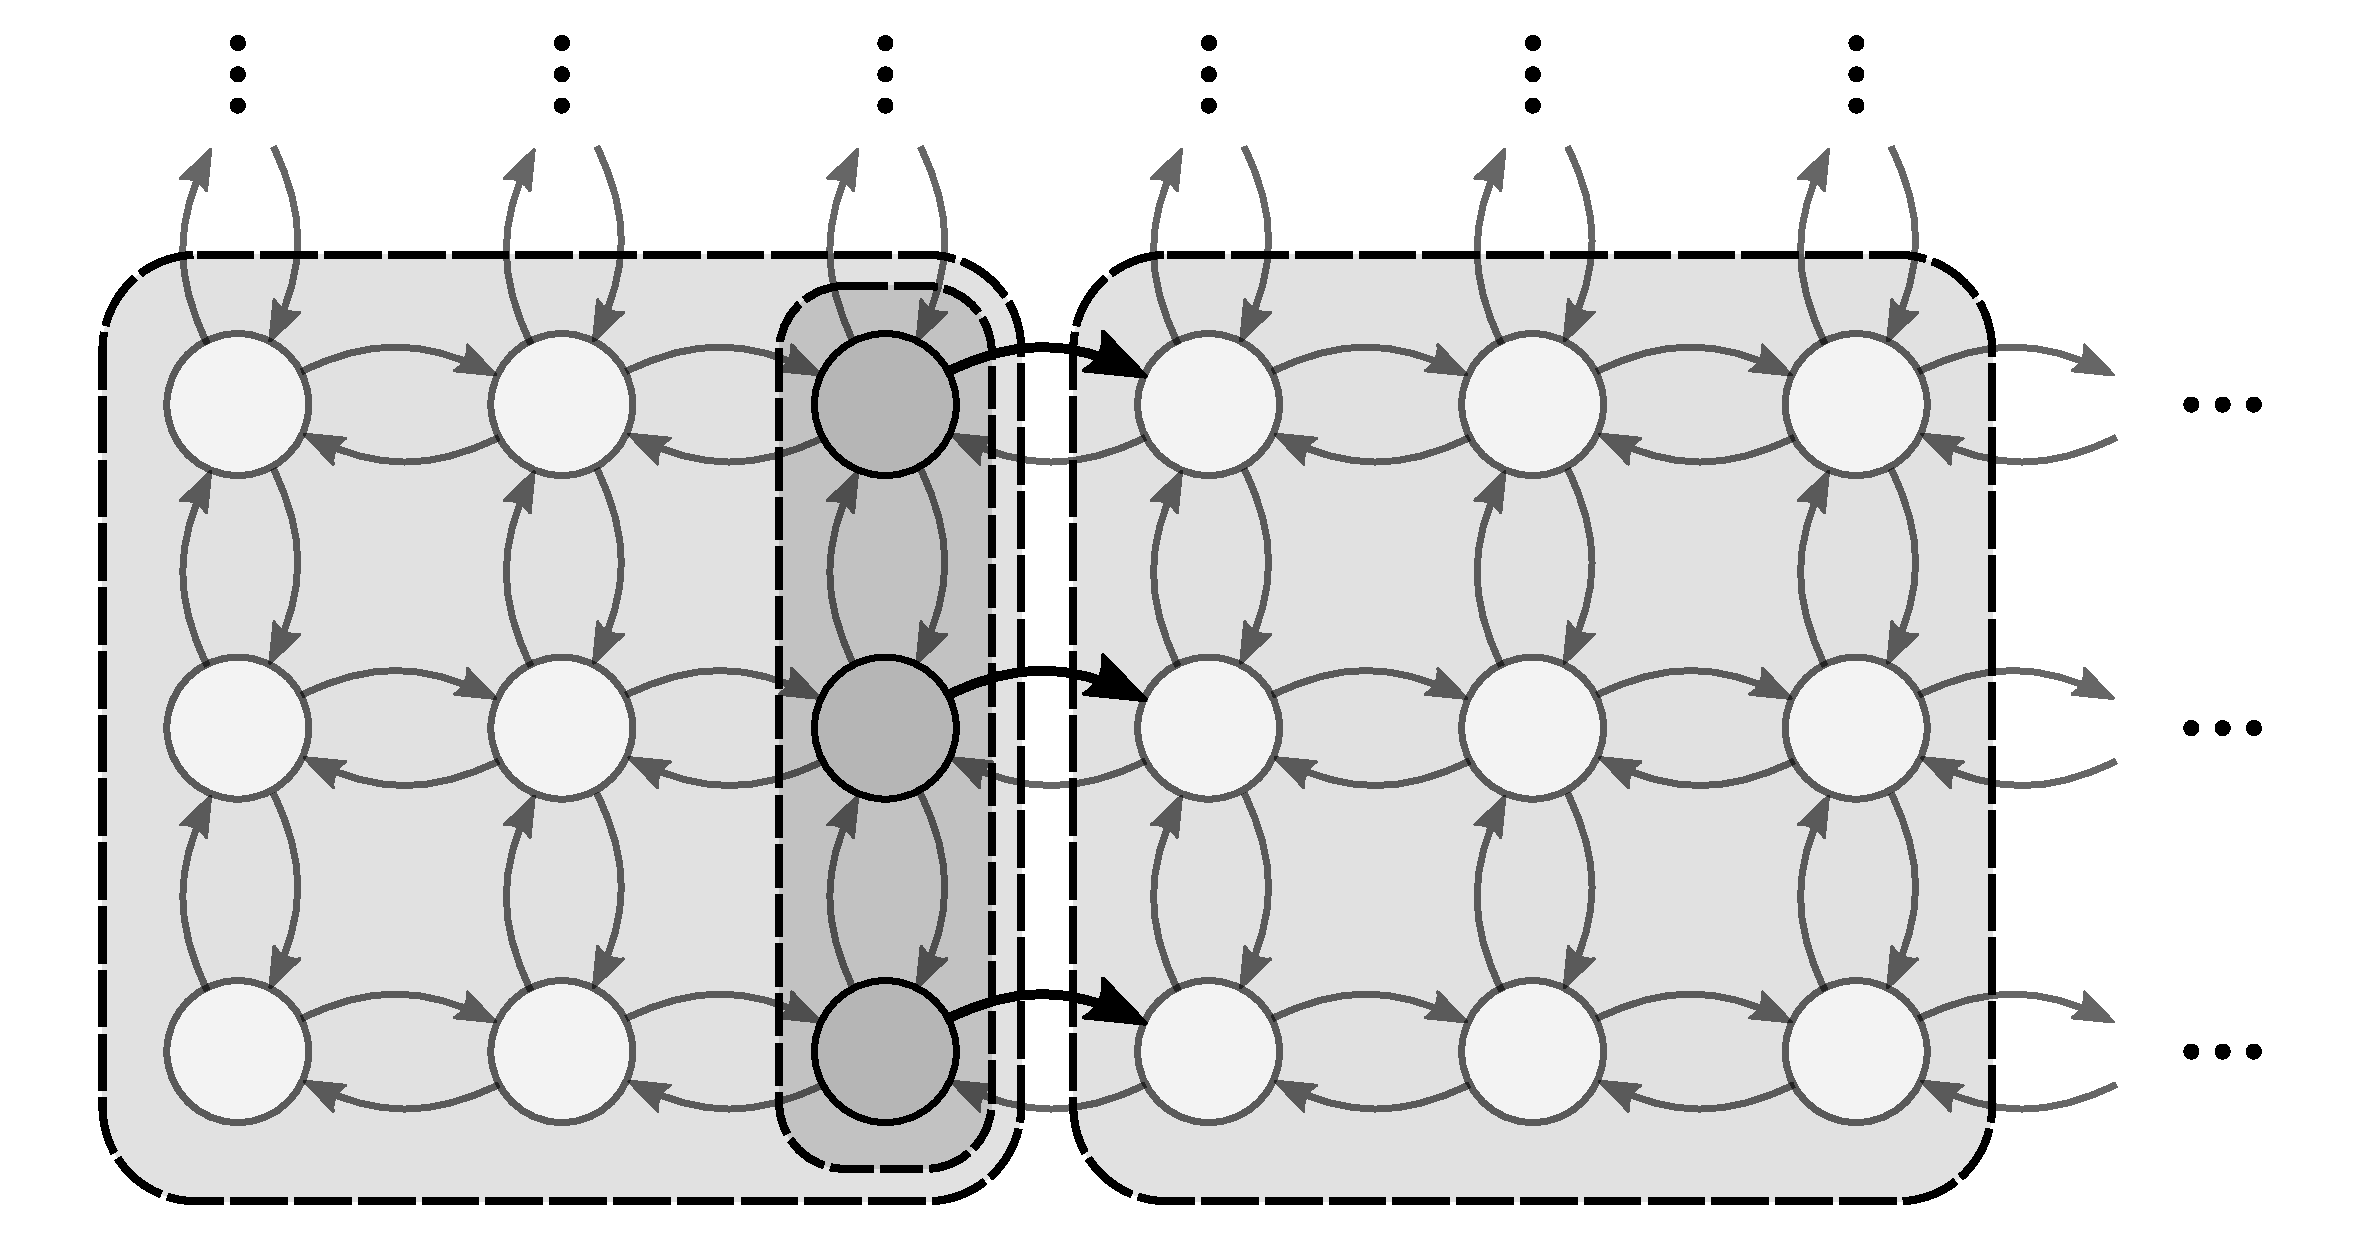
\includegraphics[width=5cm]{../gfx/macro_states.pdf}
            \end{figure}
            \begin{figure}
                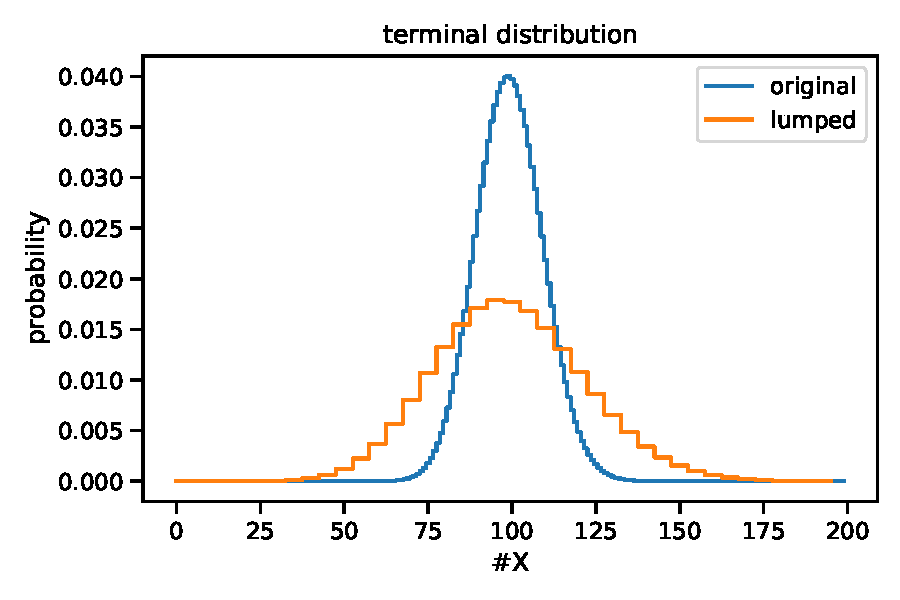
\includegraphics[scale=.3]{../gfx/lumped_dist.pdf}
            \end{figure}
        \end{column}
        \begin{column}{.6\textwidth}
            \begin{itemize}
                \item hyper-cube macro-states
                \item \emph{assumption}: uniform dist.\ within
                \item closed-form transition rates
            \end{itemize}
            \vspace{17mm}
            \begin{itemize}
                \item resulting distribution more ``flat''
                \item locate main probability mass
            \end{itemize}
            \vspace{4mm}
        \end{column}
    \end{columns}
    \bottomcite{backenkohler2020analysis,backenkohler2021abstraction}
\end{frame}

\begin{frame}{Stationary Distribution}{Finite-Space Projection}
    \begin{columns}
        \begin{column}{.30\textwidth}
            \begin{block}{Original}
                \centering
                \vspace{3mm}
                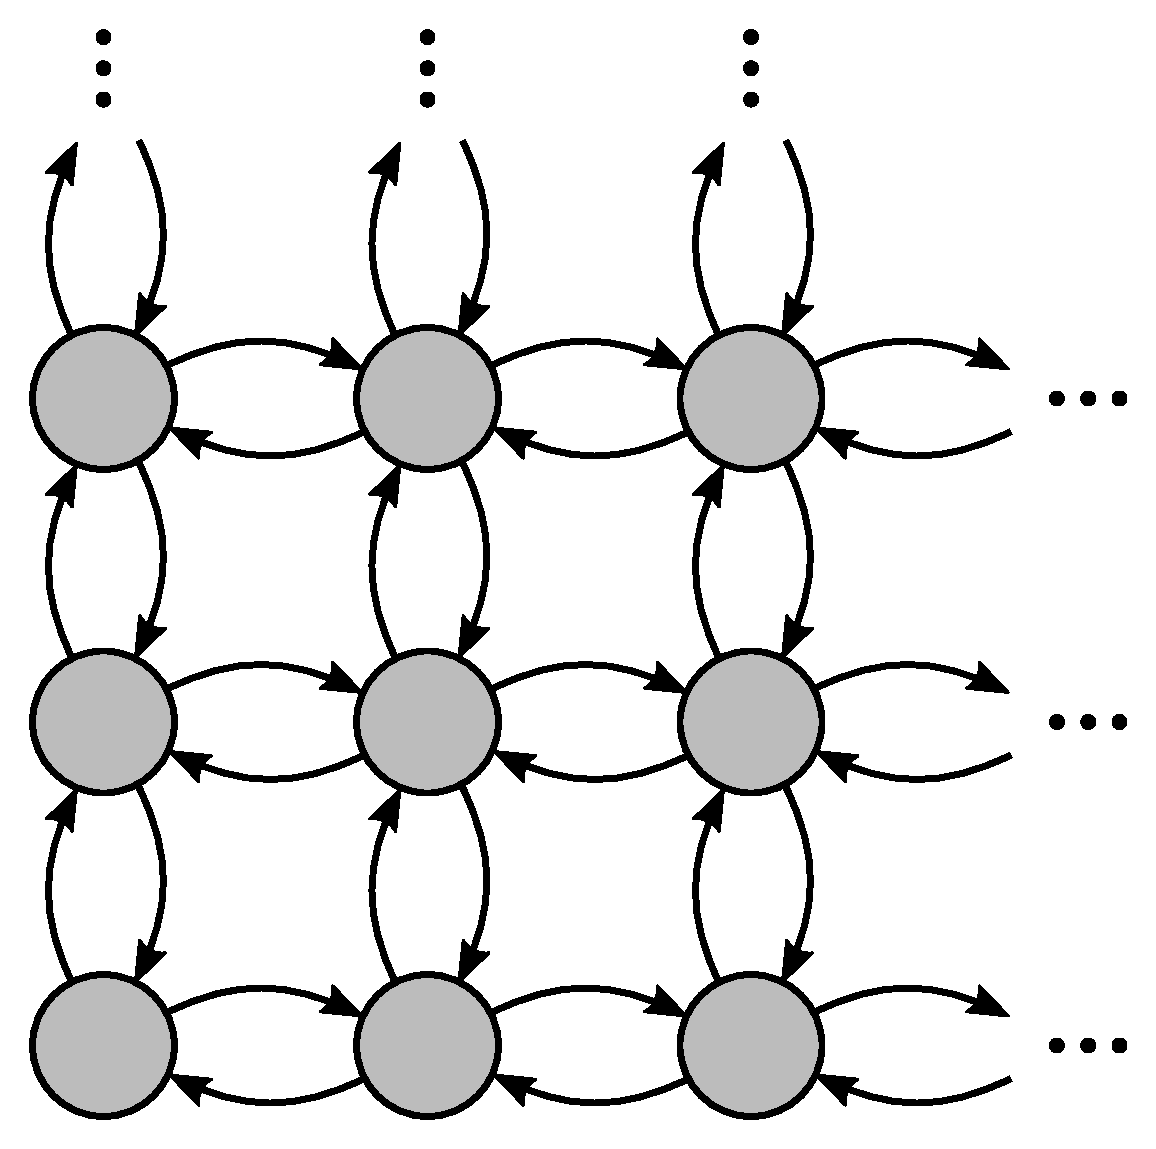
\includegraphics[height=2cm]{../gfx/state_space_untrunc.pdf}
                {\small
                \begin{itemize}
                    \item infinite
                \end{itemize}
                }
            \end{block}
        \end{column}
        \begin{column}{.30\textwidth}
            \begin{block}{Sink state}
                \centering
                \vspace{3mm}
                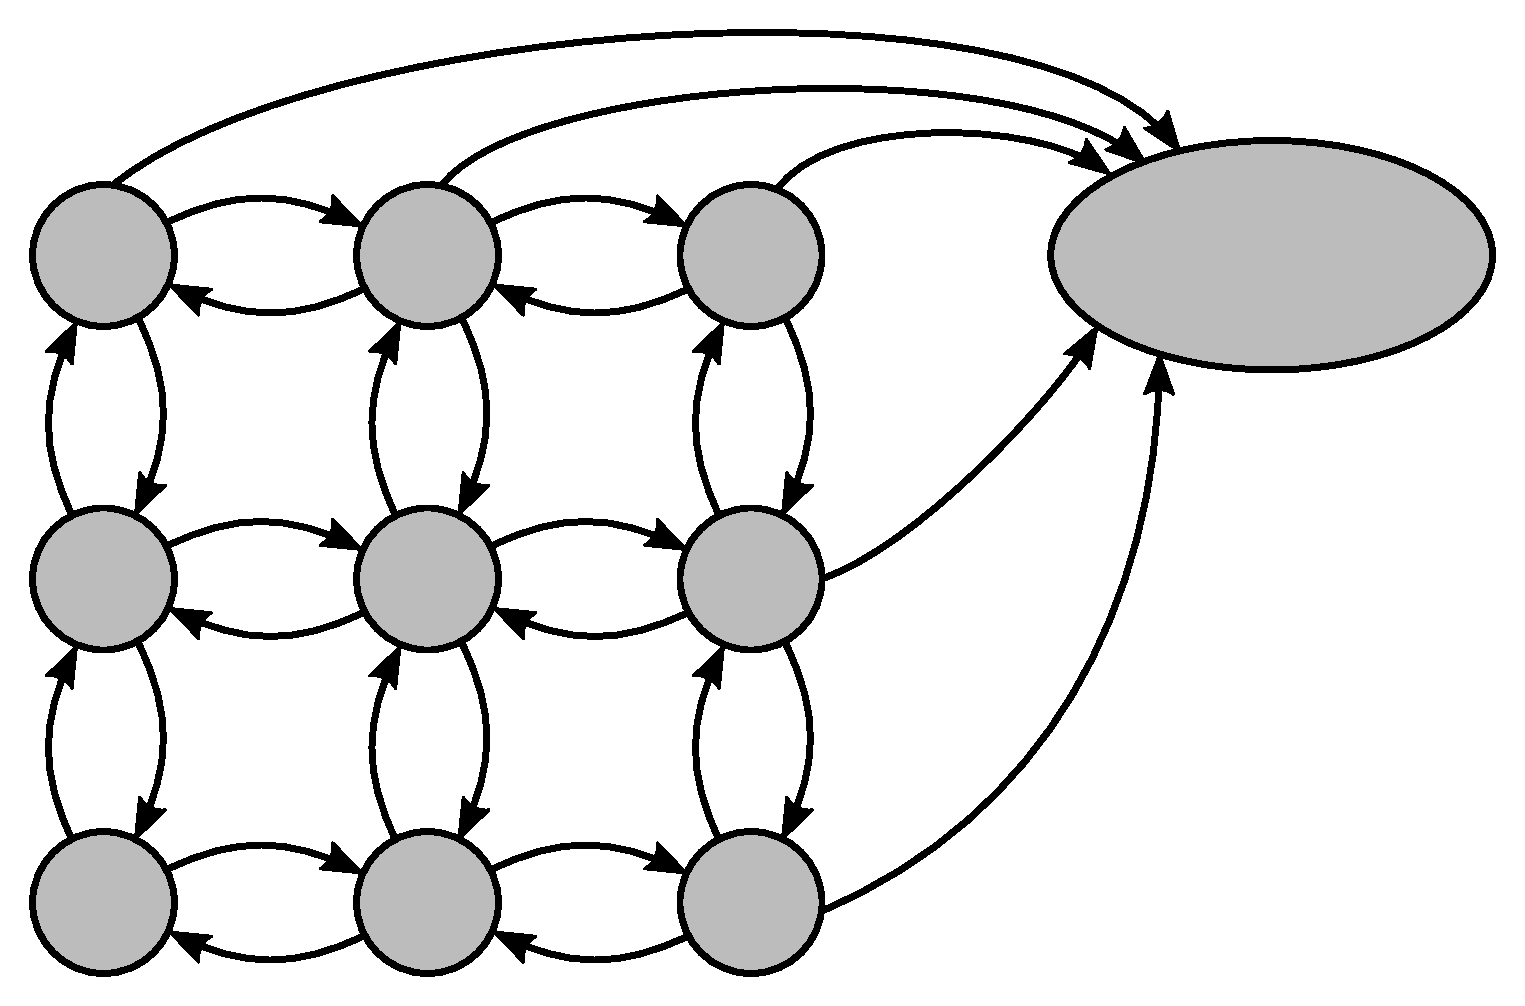
\includegraphics[height=2cm]{../gfx/state_space_redirected.pdf}
                {\small
                \begin{itemize}
                    \item transient analysis
                    \item keep track of approx.\ error
                \end{itemize}
                }
            \end{block}
        \end{column}
        \begin{column}{.30\textwidth}
            \begin{block}{Redirection}
                \centering
                \vspace{3mm}
                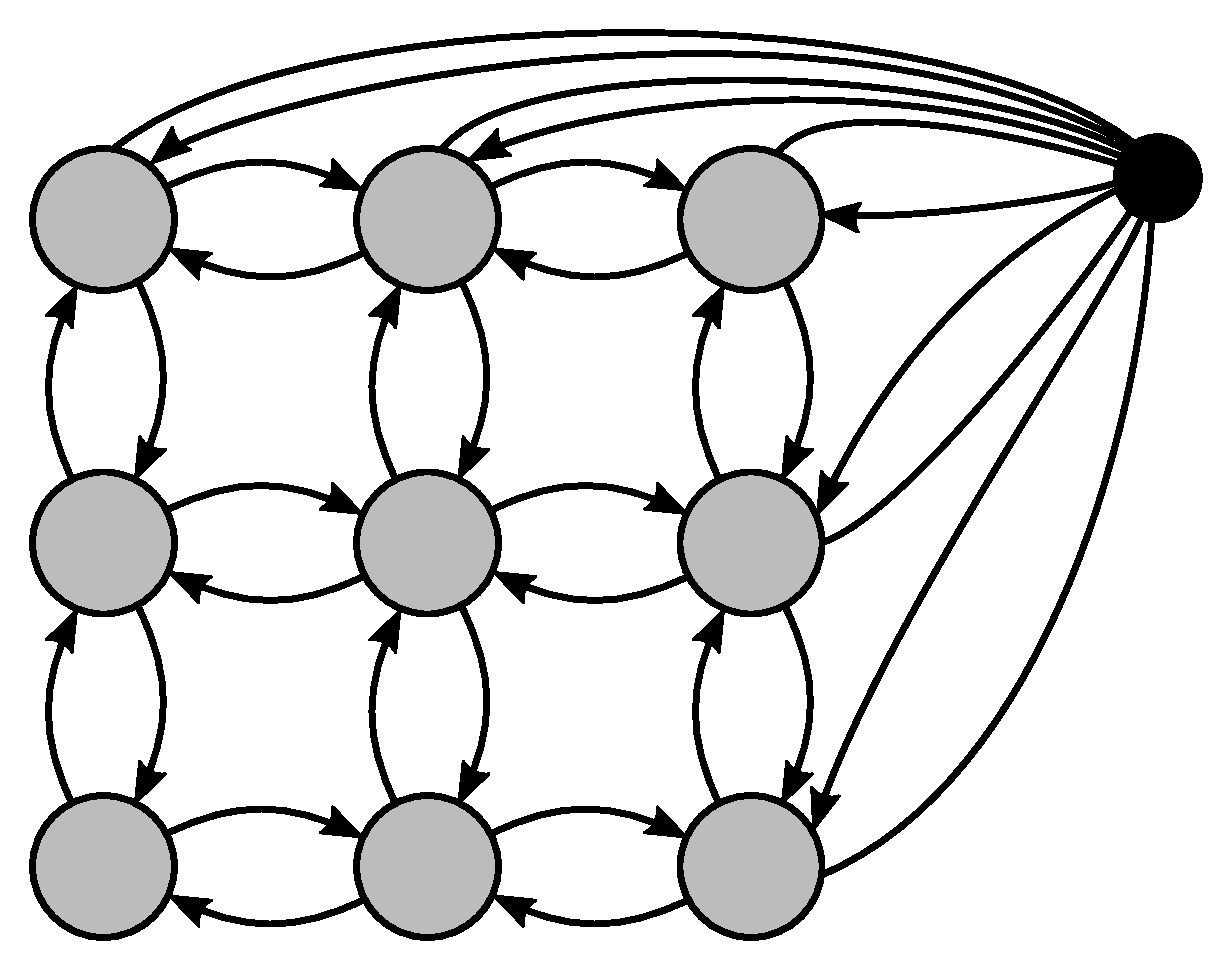
\includegraphics[height=2cm]{../gfx/state_space_reentry.pdf}
                {\small
                \begin{itemize}
                    \item stationary dist.
                    \item dependent on redirection
                \end{itemize}
                }
            \end{block}
        \end{column}
    \end{columns}
\end{frame}

\begin{frame}{Stationary Distribution}{Iterative Refinement Algorithm}
    A simple refinement based on approximate solutions:
    \begin{enumerate}
        \item start with macro-states of size $2^k$
        \item\label{itm:approx} compute approximate distribution
        \item remove states with low probability
        \item split the remaining states
        \item go to step \ref{itm:approx}
    \end{enumerate}
    \begin{figure}
        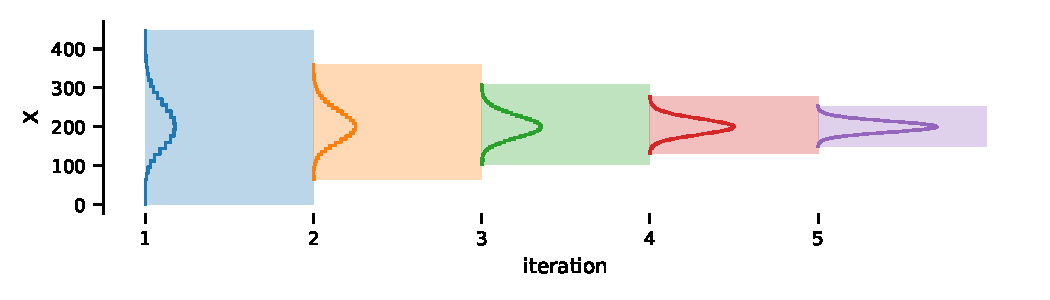
\includegraphics[width=8cm]{../gfx/bd_truncs.pdf}
    \end{figure}
    \bottomcite{backenkohler2020analysis,backenkohler2021abstraction}
\end{frame}

\begin{frame}{Bridging Problem}{Dynamical Analysis Under Initial \emph{and} Terminal Constraints}
    \begin{figure}
        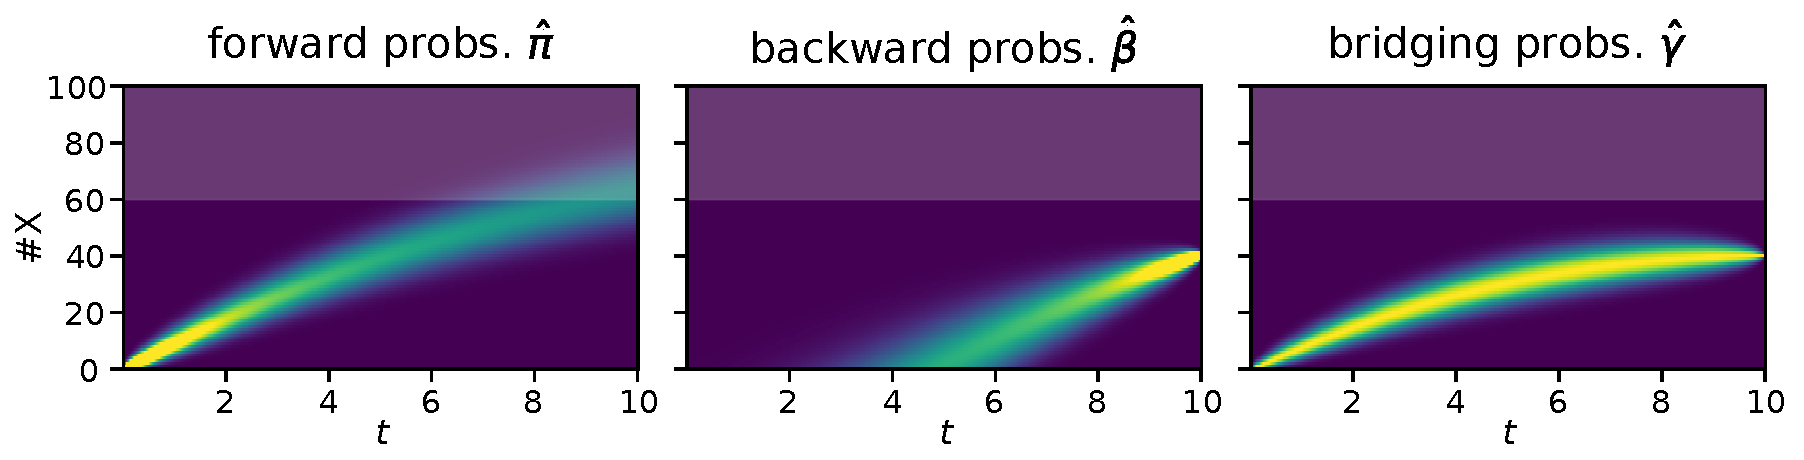
\includegraphics[width=7cm]{../gfx/bridging_bd.pdf}
    \end{figure}
    \begin{block}{Forward Probabilities}
        How the process evolves with time: $\Pr({X_t=x\mid X_0=0})$
    \end{block}
    \begin{block}{Backward Probabilities}
        Probability of ending up in a given state: $\Pr(X_T=40 \mid X_t = x)$
    \end{block}
    \begin{block}{Bridging Probabilities}
        In between: $\Pr (X_t=x\mid X_0=0, X_T=40)$
    \end{block}
    \bottomcite{backenkohler2020analysis}
\end{frame}

\begin{frame}{Bridging Problem}{Refinement}
    \bottomcite{backenkoehler2020analysis}
\end{frame}

\begin{frame}{Importance Sampling}
    
\end{frame}

\section{Conclusion}
\begin{frame}{Conclusions and Future Directions}
\end{frame}

\begin{frame}[allowframebreaks]
    \frametitle{References}
%        \bibliographystyle{amsalpha}
    \printbibliography
\end{frame}

\iffalse
\begin{frame}{Foster-Lyapunov Functions}
\end{frame}

\begin{frame}{Local Augmentation of Foster-Lyapunov Functions}
\end{frame}

\begin{frame}{Control Variates in General}
\end{frame}

\begin{frame}{Control Variates Selection Algorithm 1}
\end{frame}

\begin{frame}{Control Variates Selection Algorithm 2}
\end{frame}

\begin{frame}{Semi-definite programming}
\end{frame}
\fi

\end{document}
